Vi velger $N$ kollokasjonspunkter for et lukket legeme, og løser integrallikningen i midtpunktene mellom disse.
\begin{figure}[H]
  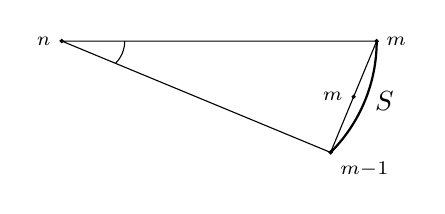
\begin{tikzpicture}
    \begin{scope}[scale = 2]
        \def\r{1}\def\smallr{.2}
        \def\thetai{-45}\def\thetaf{0}\def\thetam{180}
        \draw
            (
                {(1-\smallr)*\r*cos(\thetam) + \smallr*\r*cos(\thetaf)},
                {(1-\smallr)*\r*sin(\thetam) + \smallr*\r*sin(\thetaf)}
            ) arc (\thetaf:\thetai:\smallr) node[midway, right]{\scalebox{.6}{$\Thetatt$}};
        \draw[cap = round]
            ({\r*cos(\thetaf)}, {\r*sin(\thetaf)})--
            ({\r*cos(\thetam)}, {\r*sin(\thetam)})--
            ({\r*cos(\thetai)}, {\r*sin(\thetai)})--cycle;
        \draw[thick] ({\r*cos(\thetai)}, {\r*sin(\thetai)}) arc (\thetai:\thetaf:\r) node[midway, right]{$S$};
        \draw[fill = black] ({\r*cos(\thetaf)}, {\r*sin(\thetaf)}) circle (.01) node[right]{$\xvec_m$};
        \draw[fill = black] ({\r*cos(\thetai)}, {\r*sin(\thetai)}) circle (.01) node[below right]{$\xvec_{m-1}$};
        \draw[fill = black] ({\r*cos(\thetam)}, {\r*sin(\thetam)}) circle (.01) node[left]{$\bzhe_n$};
        \draw[fill = black]
            (
                {.5*\r*cos(\thetaf) + .5*\r*cos(\thetai)},
                {.5*\r*sin(\thetaf) + .5*\r*sin(\thetai)}
            ) circle (.01) node[left]{$\bzhe_m$};
    \end{scope}
  \end{tikzpicture}
\end{figure}

Randelementmetoden er gitt ved følgende.
\begin{itemize}
        \item Randa tilnærmes med lineære randelementer $\{S_1, \dots, S_N\}$
        \item På $S_m$ vil potensialet være konstant likt $\phi(\bzhe_m)$
        \item Potensialet løses ved invertering av systemet $\Thetatt\phi = \mathtt{h}$
\end{itemize}
